\section{Приложение}

\subsection{Приложение к теории} \label{pril_theory}
Найдём $P(\overline{k})$ из условия нормировки. При большом числе зёрен можно упростить вычисление суммы \eqref{usl_normir}, если характеризовать положение зёрен на доске Гальтона не дискретным номером ячейки, а непрерывной координатой $x$, отложенной вдоль доски. Обозначим ширину ячейки $l$, положим координату $x$ равной $x = (k - \overline{k})l$.

Введём плотность вероятностей $W(x)$ случайной координаты зерна при падении на доску. Если рассматривать интервалы $dx$, много меньшие ширины ячейки, то из связи интегральной и дифференциальной функция распределения следует, что $W(x)dx$ будет практически совпадать с вероятность того, что зерно окажется в интервале $(x, x + dx)$. Отсюда с учётом формулы \eqref{ver_formul} следует
\begin{align} \label{th:4:1}
	W(x) = \frac{P(\overline{k})}{l} \exp \left( - \frac{x^2}{2 \sigma_k^2 l^2}\right)
\end{align}

Обозначая $-x_0, x_0$ координаты крайних точек доски, получим, что условие нормировки имеет вид
\begin{align} \label{th:4:2}
	\int_{-x_0}^{x_0} { \frac{P(\overline{k})}{l}\, \exp \left( - \frac{x^2}{2 \sigma_k^2 l^2}\right) dx} = 1
\end{align}

Воспользуемся тем, что, как видно из эксперимента, при достаточно большом количестве ячеек в крайние из них попадает лишь незначительное число зёрен. На математическом языке этот факт означает, что характерный масштаб спадания плотности вероятностей \eqref{th:4:1} много меньше, чем $x_0$. Это позволяет заменить пределы интегрирования в \eqref{th:4:2} на бесконечные, в результате интеграл легко вычисляется по таблицам:
\begin{align}
	P(\overline{k}) \sqrt{2 \pi} \sigma_k = 1 
\end{align}

Из последнего равенства и следует \eqref{th:3:1}.

\subsection{Приложение к практической части} \label{pril_practic}

\subsubsection{Таблицы} \label{pril_practic_table}

\begin{center}
	\begin{longtable}{|c|c|c|c|c|c|c|c|c|c|c|c|}
		\caption[Экспериментальные данные опыта с доской Гальтона]{Экспериментальные данные опыта с доской Гальтона} \label{ap:table:1} \\
		
		 \hline

		\multicolumn{1}{|c|}{\textbf{}} &
		\multicolumn{3}{c|}{\textbf{$N = 10$}} & 
		\multicolumn{3}{c|}{\textbf{$N = N_0 / 2$}} &
		\multicolumn{3}{c|}{\textbf{$N = N_0$}} &
		\multicolumn{2}{c|}{\textbf{Среднее}} \\
		
		\hline 
		\multicolumn{1}{|c|}{\textbf{№}} &
		\multicolumn{1}{c|}{\textbf{1}} & 
		\multicolumn{1}{c|}{\textbf{2}} &
		\multicolumn{1}{c|}{\textbf{3}} &
		\multicolumn{1}{c|}{\textbf{1}} &
		\multicolumn{1}{c|}{\textbf{2}} &
		\multicolumn{1}{c|}{\textbf{3}} &
		\multicolumn{1}{c|}{\textbf{1}} &
		\multicolumn{1}{c|}{\textbf{2}} &
		\multicolumn{1}{c|}{\textbf{3}} &
		\multicolumn{1}{c|}{\textbf{$N = N_0 / 2$}} &
		\multicolumn{1}{c|}{\textbf{$N = N_0$}}\\ \hline 
		
		\endfirsthead
		
		\multicolumn{12}{c}%
		{{ \tablename\ \thetable{} -- продолжение с предыдущей страницы}} \\
		\hline
		
		\multicolumn{1}{|c|}{\textbf{}} &
		\multicolumn{3}{c|}{\textbf{$N = 10$}} & 
		\multicolumn{3}{c|}{\textbf{$N = N_0 / 2$}} &
		\multicolumn{3}{c|}{\textbf{$N = N_0$}} &
		\multicolumn{2}{c|}{\textbf{Среднее}} \\
		 
		\hline
		\multicolumn{1}{|c|}{\textbf{№}} &
		\multicolumn{1}{c|}{\textbf{1}} & 
		\multicolumn{1}{c|}{\textbf{2}} &
		\multicolumn{1}{c|}{\textbf{3}} &
		\multicolumn{1}{c|}{\textbf{1}} &
		\multicolumn{1}{c|}{\textbf{2}} &
		\multicolumn{1}{c|}{\textbf{3}} &
		\multicolumn{1}{c|}{\textbf{1}} &
		\multicolumn{1}{c|}{\textbf{2}} &
		\multicolumn{1}{c|}{\textbf{3}} &
		\multicolumn{1}{c|}{\textbf{$N = N_0 / 2$}} &
		\multicolumn{1}{c|}{\textbf{$N = N_0$}}\\ \hline 
		\endhead
		
		\hline \multicolumn{12}{|l|}{{Продолжение на следующей странице}} \\ \hline
		\endfoot
		
		\hline \hline
		\endlastfoot
		
		1  & 0 & 0 & 0 & 0  & 0  & 0  & 0   & 0   & 0   & 0,0      & 0,0    \\ \hline
		2  & 0 & 0 & 0 & 0  & 0  & 0  & 0   & 0   & 0   & 0,0      & 0,0    \\ \hline
		3  & 0 & 0 & 0 & 0  & 0  & 0  & 0   & 0   & 0   & 0,0      & 0,0    \\ \hline
		4  & 0 & 0 & 0 & 0  & 0  & 0  & 0   & 0   & 0   & 0,0      & 0,0    \\ \hline
		5  & 0 & 0 & 0 & 0  & 0  & 0  & 0   & 0   & 0   & 0,0      & 0,0    \\ \hline
		6  & 0 & 0 & 0 & 0  & 1  & 0  & 2   & 2   & 2   & 1,2      & 2,0    \\ \hline
		7  & 0 & 0 & 0 & 0  & 1  & 0  & 3   & 3   & 4   & 1,8      & 3,3    \\ \hline
		8  & 0 & 0 & 0 & 4  & 2  & 3  & 4   & 5   & 4   & 3,7      & 4,3    \\ \hline
		9  & 0 & 0 & 0 & 5  & 3  & 4  & 7   & 7   & 5   & 5,2      & 6,3    \\ \hline
		10 & 0 & 0 & 0 & 5  & 4  & 4  & 9   & 8   & 7   & 6,2      & 8,0    \\ \hline
		11 & 1 & 0 & 0 & 8  & 7  & 5  & 12  & 11  & 10  & 8,8      & 11,0   \\ \hline
		12 & 0 & 0 & 0 & 7  & 8  & 8  & 17  & 14  & 13  & 11,2     & 14,7   \\ \hline
		13 & 0 & 0 & 0 & 10 & 9  & 10 & 19  & 18  & 16  & 13,7     & 17,7   \\ \hline
		14 & 0 & 0 & 0 & 11 & 12 & 10 & 22  & 21  & 20  & 16,0     & 21,0   \\ \hline
		15 & 0 & 0 & 0 & 15 & 15 & 15 & 25  & 28  & 28  & 21,0     & 27,0   \\ \hline
		16 & 0 & 0 & 0 & 17 & 17 & 16 & 35  & 34  & 30  & 24,8     & 33,0   \\ \hline
		17 & 0 & 0 & 0 & 20 & 22 & 20 & 44  & 44  & 39  & 31,5     & 42,3   \\ \hline
		18 & 0 & 0 & 0 & 19 & 23 & 24 & 47  & 50  & 44  & 34,5     & 47,0   \\ \hline
		19 & 0 & 0 & 0 & 25 & 27 & 25 & 54  & 57  & 51  & 39,8     & 54,0   \\ \hline
		20 & 0 & 0 & 1 & 33 & 31 & 33 & 66  & 62  & 65  & 48,3     & 64,3   \\ \hline
		21 & 1 & 0 & 0 & 35 & 34 & 35 & 69  & 78  & 70  & 53,5     & 72,3   \\ \hline
		22 & 0 & 1 & 1 & 35 & 35 & 37 & 75  & 71  & 68  & 53,5     & 71,3   \\ \hline
		23 & 0 & 4 & 0 & 40 & 42 & 40 & 84  & 84  & 85  & 62,5     & 84,3   \\ \hline
		24 & 1 & 2 & 0 & 41 & 46 & 41 & 88  & 93  & 88  & 66,2     & 89,7   \\ \hline
		25 & 1 & 0 & 0 & 47 & 48 & 45 & 98  & 99  & 100 & 72,8     & 99,0   \\ \hline
		26 & 0 & 0 & 1 & 42 & 45 & 47 & 96  & 94  & 96  & 70,0     & 95,3   \\ \hline
		27 & 1 & 0 & 0 & 48 & 46 & 50 & 98  & 98  & 97  & 72,8     & 97,7   \\ \hline
		28 & 0 & 0 & 2 & 50 & 50 & 48 & 103 & 104 & 102 & 76,2     & 103,0  \\ \hline
		29 & 1 & 1 & 0 & 52 & 50 & 50 & 100 & 98  & 98  & 74,7     & 98,7   \\ \hline
		30 & 0 & 0 & 0 & 45 & 48 & 46 & 95  & 96  & 95  & 70,8     & 95,3   \\ \hline
		31 & 0 & 0 & 1 & 43 & 45 & 43 & 91  & 90  & 91  & 67,2     & 90,7   \\ \hline
		32 & 2 & 0 & 0 & 40 & 46 & 40 & 89  & 85  & 87  & 64,5     & 87,0   \\ \hline
		33 & 0 & 1 & 1 & 35 & 36 & 37 & 76  & 79  & 79  & 57,0     & 78,0   \\ \hline
		34 & 0 & 0 & 0 & 39 & 35 & 35 & 75  & 75  & 75  & 55,7     & 75,0   \\ \hline
		35 & 1 & 0 & 0 & 25 & 30 & 29 & 60  & 63  & 65  & 45,3     & 62,7   \\ \hline
		36 & 0 & 0 & 1 & 27 & 25 & 27 & 58  & 55  & 55  & 41,2     & 56,0   \\ \hline
		37 & 1 & 1 & 1 & 25 & 23 & 25 & 50  & 49  & 50  & 37,0     & 49,7   \\ \hline
		38 & 0 & 0 & 1 & 20 & 17 & 20 & 40  & 35  & 38  & 28,3     & 37,7   \\ \hline
		39 & 0 & 0 & 0 & 15 & 14 & 15 & 33  & 29  & 35  & 23,5     & 32,3   \\ \hline
		40 & 0 & 0 & 0 & 15 & 13 & 18 & 29  & 28  & 30  & 22,2     & 29,0   \\ \hline
		41 & 0 & 0 & 0 & 10 & 12 & 10 & 22  & 23  & 22  & 16,5     & 22,3   \\ \hline
		42 & 0 & 0 & 0 & 8  & 7  & 7  & 18  & 17  & 18  & 12,5     & 17,7   \\ \hline
		43 & 0 & 0 & 0 & 7  & 6  & 6  & 15  & 15  & 17  & 11,0     & 15,7   \\ \hline
		44 & 0 & 0 & 0 & 5  & 5  & 5  & 10  & 9   & 10  & 7,3      & 9,7    \\ \hline
		45 & 0 & 0 & 0 & 4  & 3  & 3  & 8   & 8   & 10  & 6,0      & 8,7    \\ \hline
		46 & 0 & 0 & 0 & 3  & 4  & 3  & 5   & 6   & 5   & 4,3      & 5,3    \\ \hline
		47 & 0 & 0 & 0 & 0  & 0  & 0  & 4   & 4   & 3   & 1,8      & 3,7    \\ \hline
		48 & 0 & 0 & 0 & 0  & 0  & 0  & 4   & 3   & 2   & 1,5      & 3,0    \\ \hline
		49 & 0 & 0 & 0 & 0  & 0  & 0  & 2   & 3   & 2   & 1,2      & 2,3    \\ \hline
		50 & 0 & 0 & 0 & 0  & 0  & 0  & 1   & 2   & 0   & 0,5      & 1,0    \\ \hline
		51 & 0 & 0 & 0 & 0  & 0  & 0  & 0   & 0   & 0   & 0,0      & 0,0    \\ \hline
		52 & 0 & 0 & 0 & 0  & 0  & 0  & 0   & 0   & 0   & 0,0      & 0,0    \\ \hline
		53 & 0 & 0 & 0 & 0  & 0  & 0  & 0   & 0   & 0   & 0,0      & 0,0    \\ \hline
		54 & 0 & 0 & 0 & 0  & 0  & 0  & 0   & 0   & 0   & 0,0      & 0,0    \\ 
	\end{longtable}
\end{center}


\begin{center}
	\begin{longtable}{|c|c||c|c||c|c||c|c|}
		\caption[Экспериментальные данные опыта с доской Гальтона]{Экспериментальные данные опыта с измерением сопротивления (общий вид)} \label{ap:table:2} \\
		
		\hline
		
		\multicolumn{1}{|c|}{\textbf{№}} &
		\multicolumn{1}{c||}{\textbf{R, Ом}} & 
		\multicolumn{1}{c|}{\textbf{№}} &
		\multicolumn{1}{c||}{\textbf{R, Ом}} &
		\multicolumn{1}{c|}{\textbf{№}} &
		\multicolumn{1}{c||}{\textbf{R, Ом}} &
		\multicolumn{1}{c|}{\textbf{№}} &
		\multicolumn{1}{c|}{\textbf{R, Ом}} \\ \hline
		
		\endfirsthead
		
		\multicolumn{8}{c}%
		{{ \tablename\ \thetable{} -- продолжение с предыдущей страницы}} \\
		\hline
		
		\multicolumn{1}{|c|}{\textbf{№}} &
		\multicolumn{1}{c|}{\textbf{R, Ом}} & 
		\multicolumn{1}{c|}{\textbf{№}} &
		\multicolumn{1}{c|}{\textbf{R, Ом}} &
		\multicolumn{1}{|c|}{\textbf{№}} &
		\multicolumn{1}{c|}{\textbf{R, Ом}} &
		\multicolumn{1}{|c|}{\textbf{№}} &
		\multicolumn{1}{c|}{\textbf{R, Ом}} \\
		
		\endhead
		
		\hline \multicolumn{8}{|l|}{{Продолжение на следующей странице}} \\ \hline
		\endfoot
		
		\hline \hline
		\endlastfoot
		
		1  & 475 & 26 & 508 & 51 & 511 & 76  & 515 \\ \hline
		2  & 485 & 27 & 508 & 52 & 511 & 77  & 516 \\ \hline
		3  & 488 & 28 & 508 & 53 & 511 & 78  & 516 \\ \hline
		4  & 496 & 29 & 508 & 54 & 512 & 79  & 516 \\ \hline
		5  & 496 & 30 & 509 & 55 & 512 & 80  & 516 \\ \hline
		6  & 497 & 31 & 509 & 56 & 512 & 81  & 516 \\ \hline
		7  & 498 & 32 & 509 & 57 & 512 & 82  & 516 \\ \hline
		8  & 499 & 33 & 509 & 58 & 512 & 83  & 518 \\ \hline
		9  & 499 & 34 & 509 & 59 & 513 & 84  & 518 \\ \hline
		10 & 501 & 35 & 509 & 60 & 513 & 85  & 519 \\ \hline
		11 & 501 & 36 & 509 & 61 & 513 & 86  & 519 \\ \hline
		12 & 502 & 37 & 509 & 62 & 513 & 87  & 519 \\ \hline
		13 & 502 & 38 & 509 & 63 & 513 & 88  & 519 \\ \hline
		14 & 504 & 39 & 510 & 64 & 513 & 89  & 520 \\ \hline
		15 & 505 & 40 & 510 & 65 & 513 & 90  & 521 \\ \hline
		16 & 505 & 41 & 510 & 66 & 513 & 91  & 521 \\ \hline
		17 & 506 & 42 & 510 & 67 & 514 & 92  & 521 \\ \hline
		18 & 506 & 43 & 510 & 68 & 514 & 93  & 524 \\ \hline
		19 & 507 & 44 & 510 & 69 & 514 & 94  & 524 \\ \hline
		20 & 507 & 45 & 510 & 70 & 514 & 95  & 527 \\ \hline
		21 & 507 & 46 & 510 & 71 & 514 & 96  & 528 \\ \hline
		22 & 507 & 47 & 510 & 72 & 514 & 97  & 529 \\ \hline
		23 & 507 & 48 & 510 & 73 & 515 & 98  & 539 \\ \hline
		24 & 507 & 49 & 510 & 74 & 515 & 99  & 543 \\ \hline
		25 & 508 & 50 & 511 & 75 & 515 & 100 & 545 \\ 
	\end{longtable}
\end{center}


\begin{center}
	\begin{longtable}{|c|c|c||c|c|c|}
		\caption[Экспериментальные данные]{Экспериментальные данные опыта с измерением сопротивления (Обработанные)} \label{ap:table:3} \\
		\hline
		\multicolumn{1}{|c|}{\textbf{№}} &
		\multicolumn{1}{c|}{\textbf{R, Ом}} & 
		\multicolumn{1}{c||}{\textbf{Количество}} &
		\multicolumn{1}{c|}{\textbf{№}} &
		\multicolumn{1}{c|}{\textbf{R, Ом}} & 
		\multicolumn{1}{c|}{\textbf{Количество}} \\ \hline
		\endfirsthead
		
		1  & 475 & 1  & 18 & 512 & 5 \\ \hline
		2  & 485 & 1  & 19 & 513 & 8 \\ \hline
		3  & 488 & 1  & 20 & 514 & 6 \\ \hline
		4  & 496 & 2  & 21 & 515 & 4 \\ \hline
		5  & 497 & 1  & 22 & 516 & 6 \\ \hline
		6  & 498 & 1  & 23 & 518 & 2 \\ \hline
		7  & 499 & 2  & 24 & 519 & 4 \\ \hline
		8  & 501 & 2  & 25 & 520 & 1 \\ \hline
		9  & 502 & 2  & 26 & 521 & 3 \\ \hline
		10 & 504 & 1  & 27 & 524 & 2 \\ \hline
		11 & 505 & 2  & 28 & 527 & 1 \\ \hline
		12 & 506 & 2  & 29 & 528 & 1 \\ \hline
		13 & 507 & 6  & 30 & 529 & 1 \\ \hline
		14 & 508 & 5  & 31 & 539 & 1 \\ \hline
		15 & 509 & 9  & 32 & 543 & 1 \\ \hline
		16 & 510 & 11 & 33 & 545 & 1 \\ \hline
		17 & 511 & 4  &    &     &   \\ \hline
		
		
	\end{longtable}
\end{center}

\newpage

\subsubsection{Графики} \label{pril_practic_graph}

\begin{figure} [H]
	\centering
	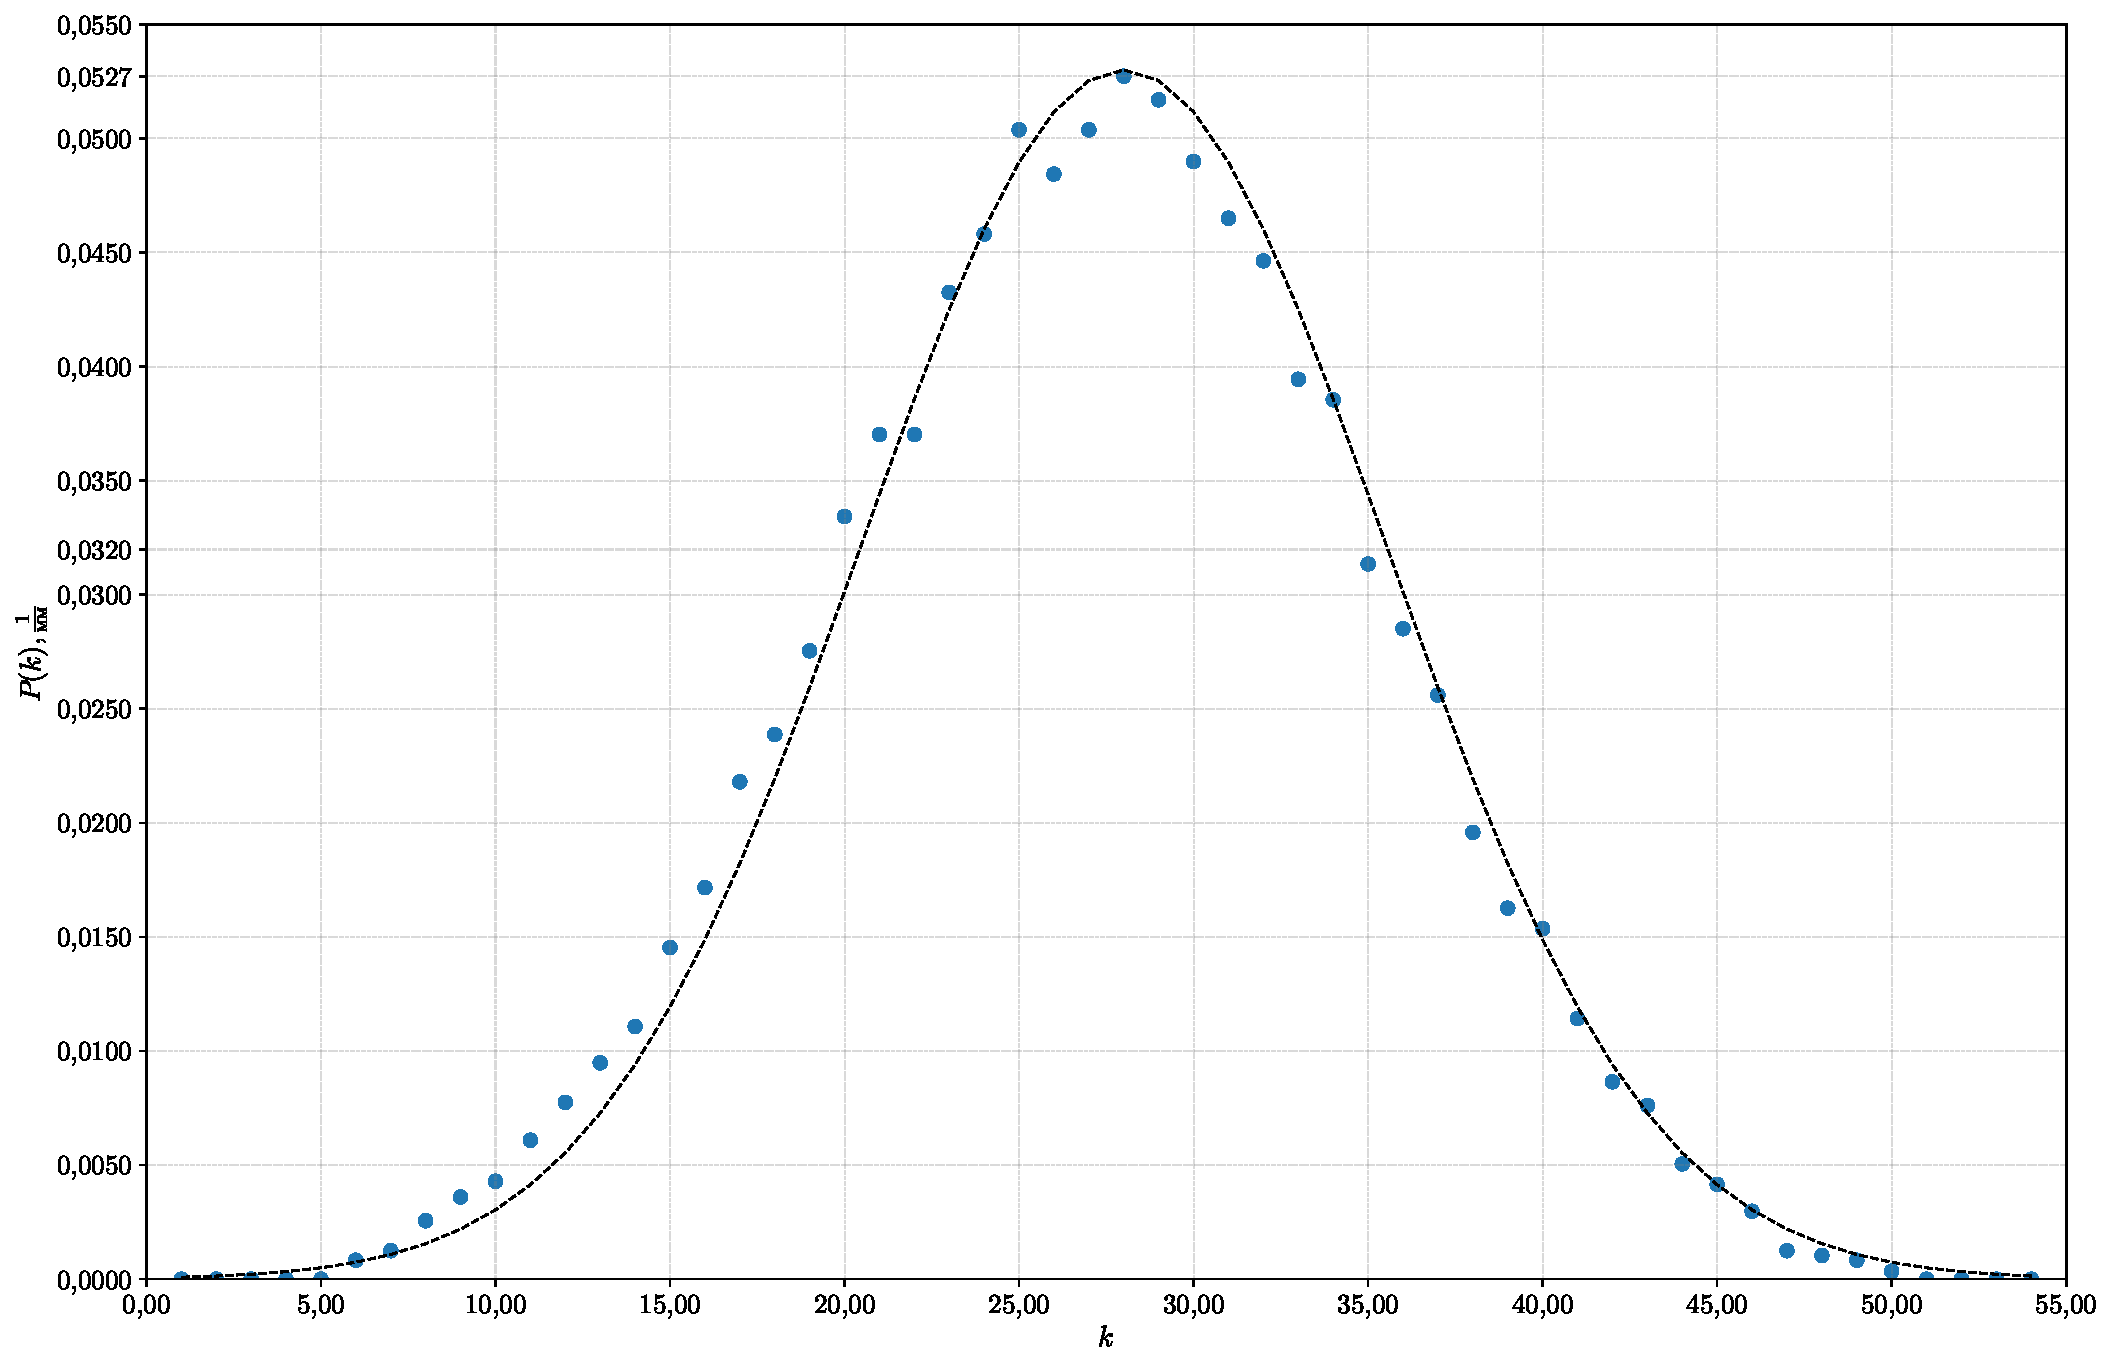
\includegraphics[angle = 270, width=0.8\textwidth]{ graph_1 } 
	\caption{График для $N = N_0/2$}
	
	 \label{fig:graph-1}
\end{figure}

\begin{figure}[H] 
	\centering
	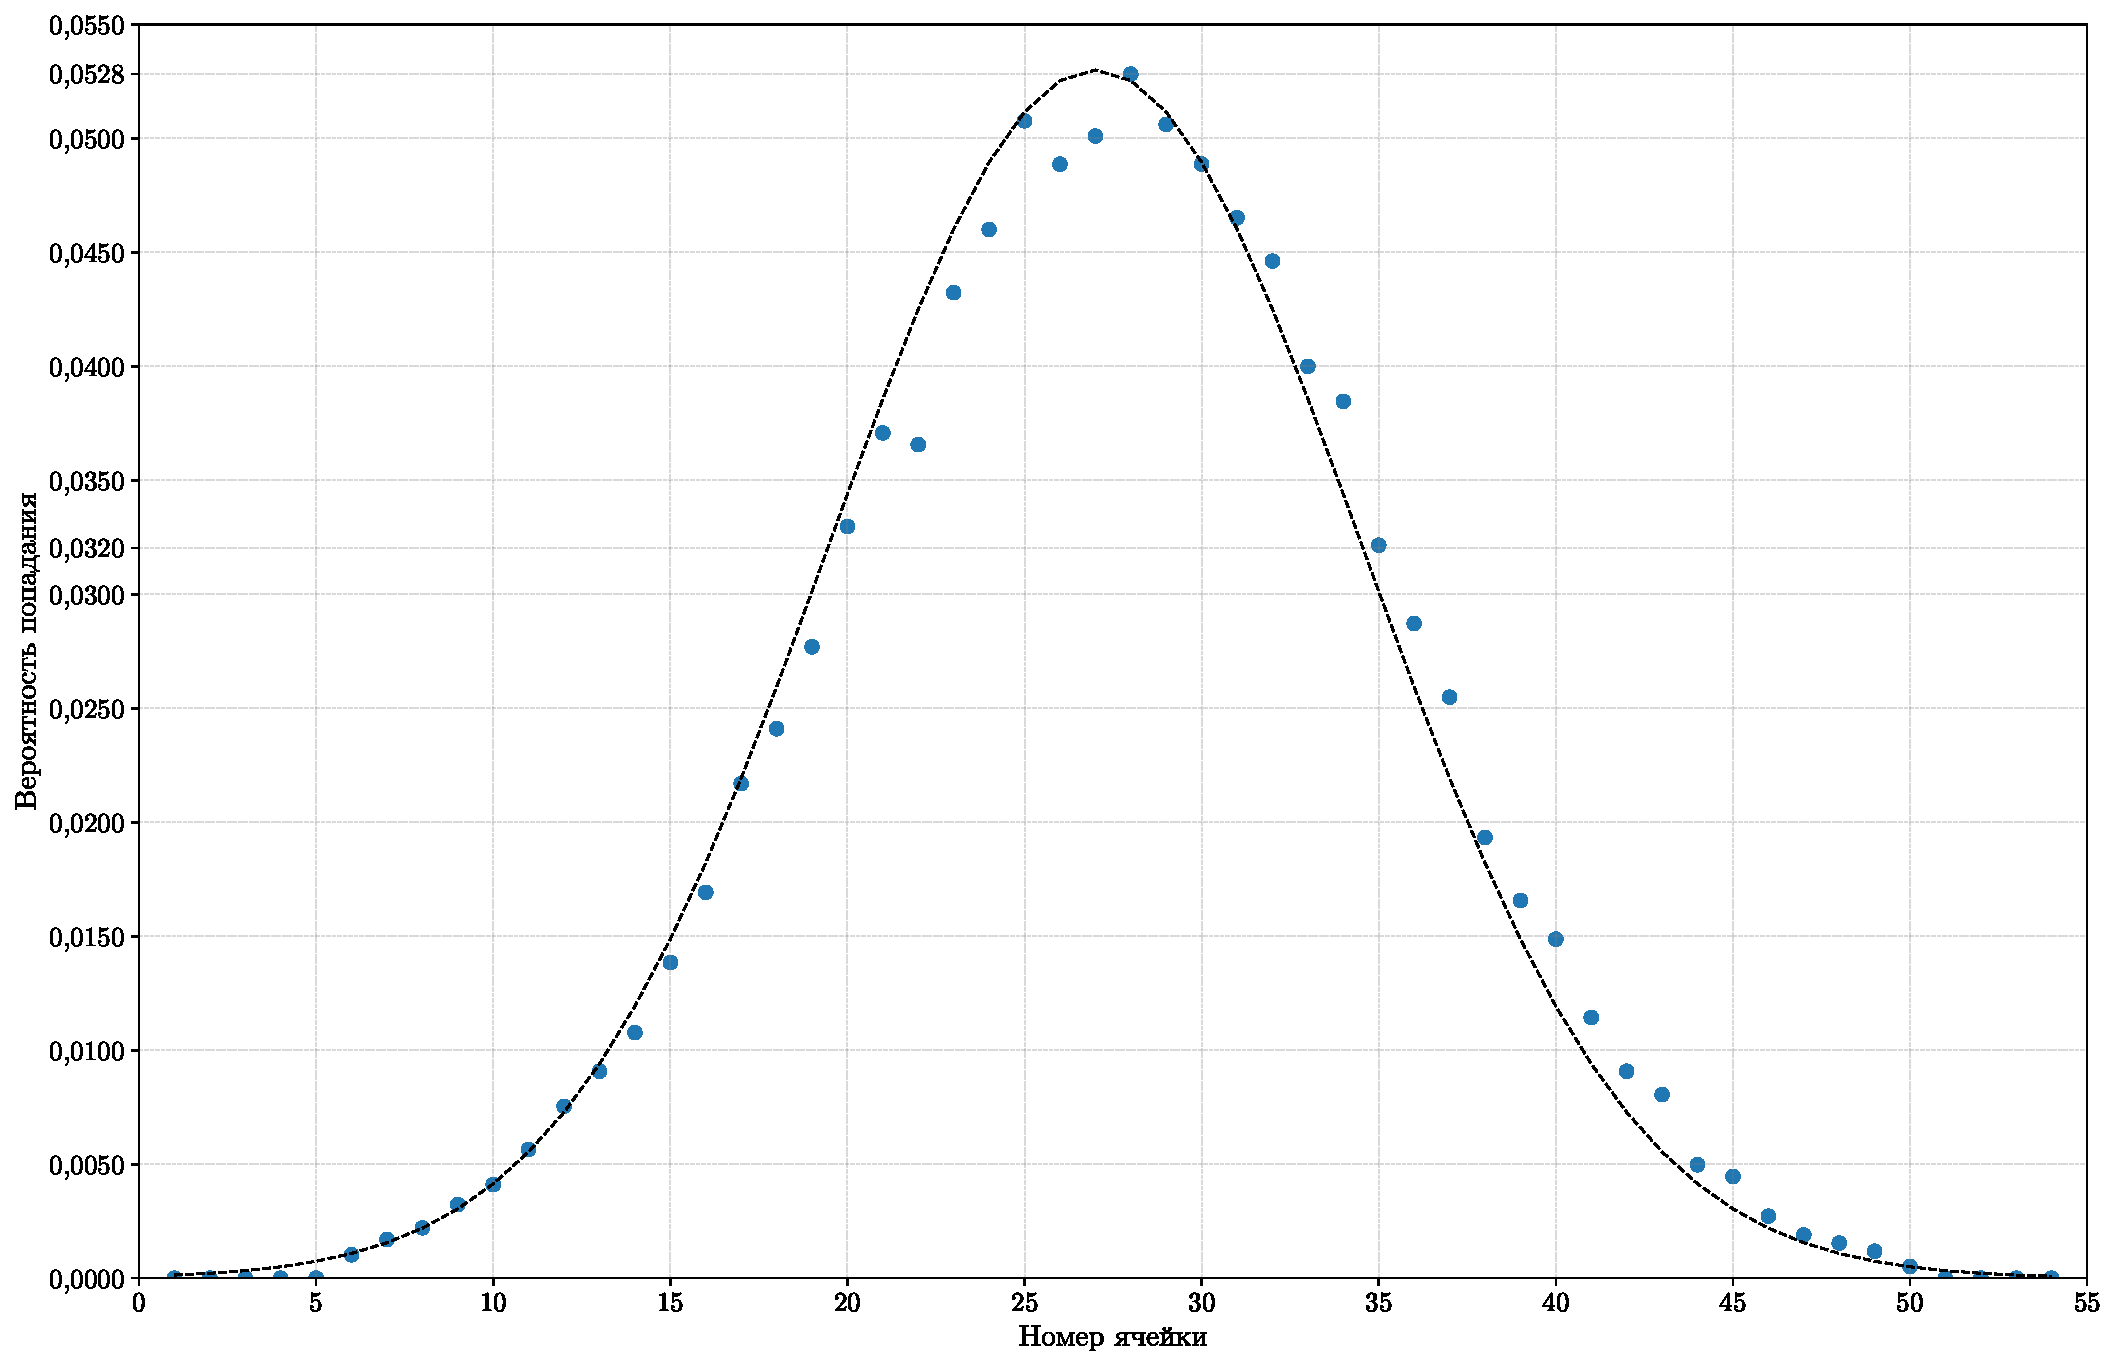
\includegraphics[angle = 270, width=0.8\textwidth]{ graph_2 } 
	\caption{График для $N = N_0$}
	
	\label{fig:graph-2} 
\end{figure}

\begin{figure}[H] 
	\centering
	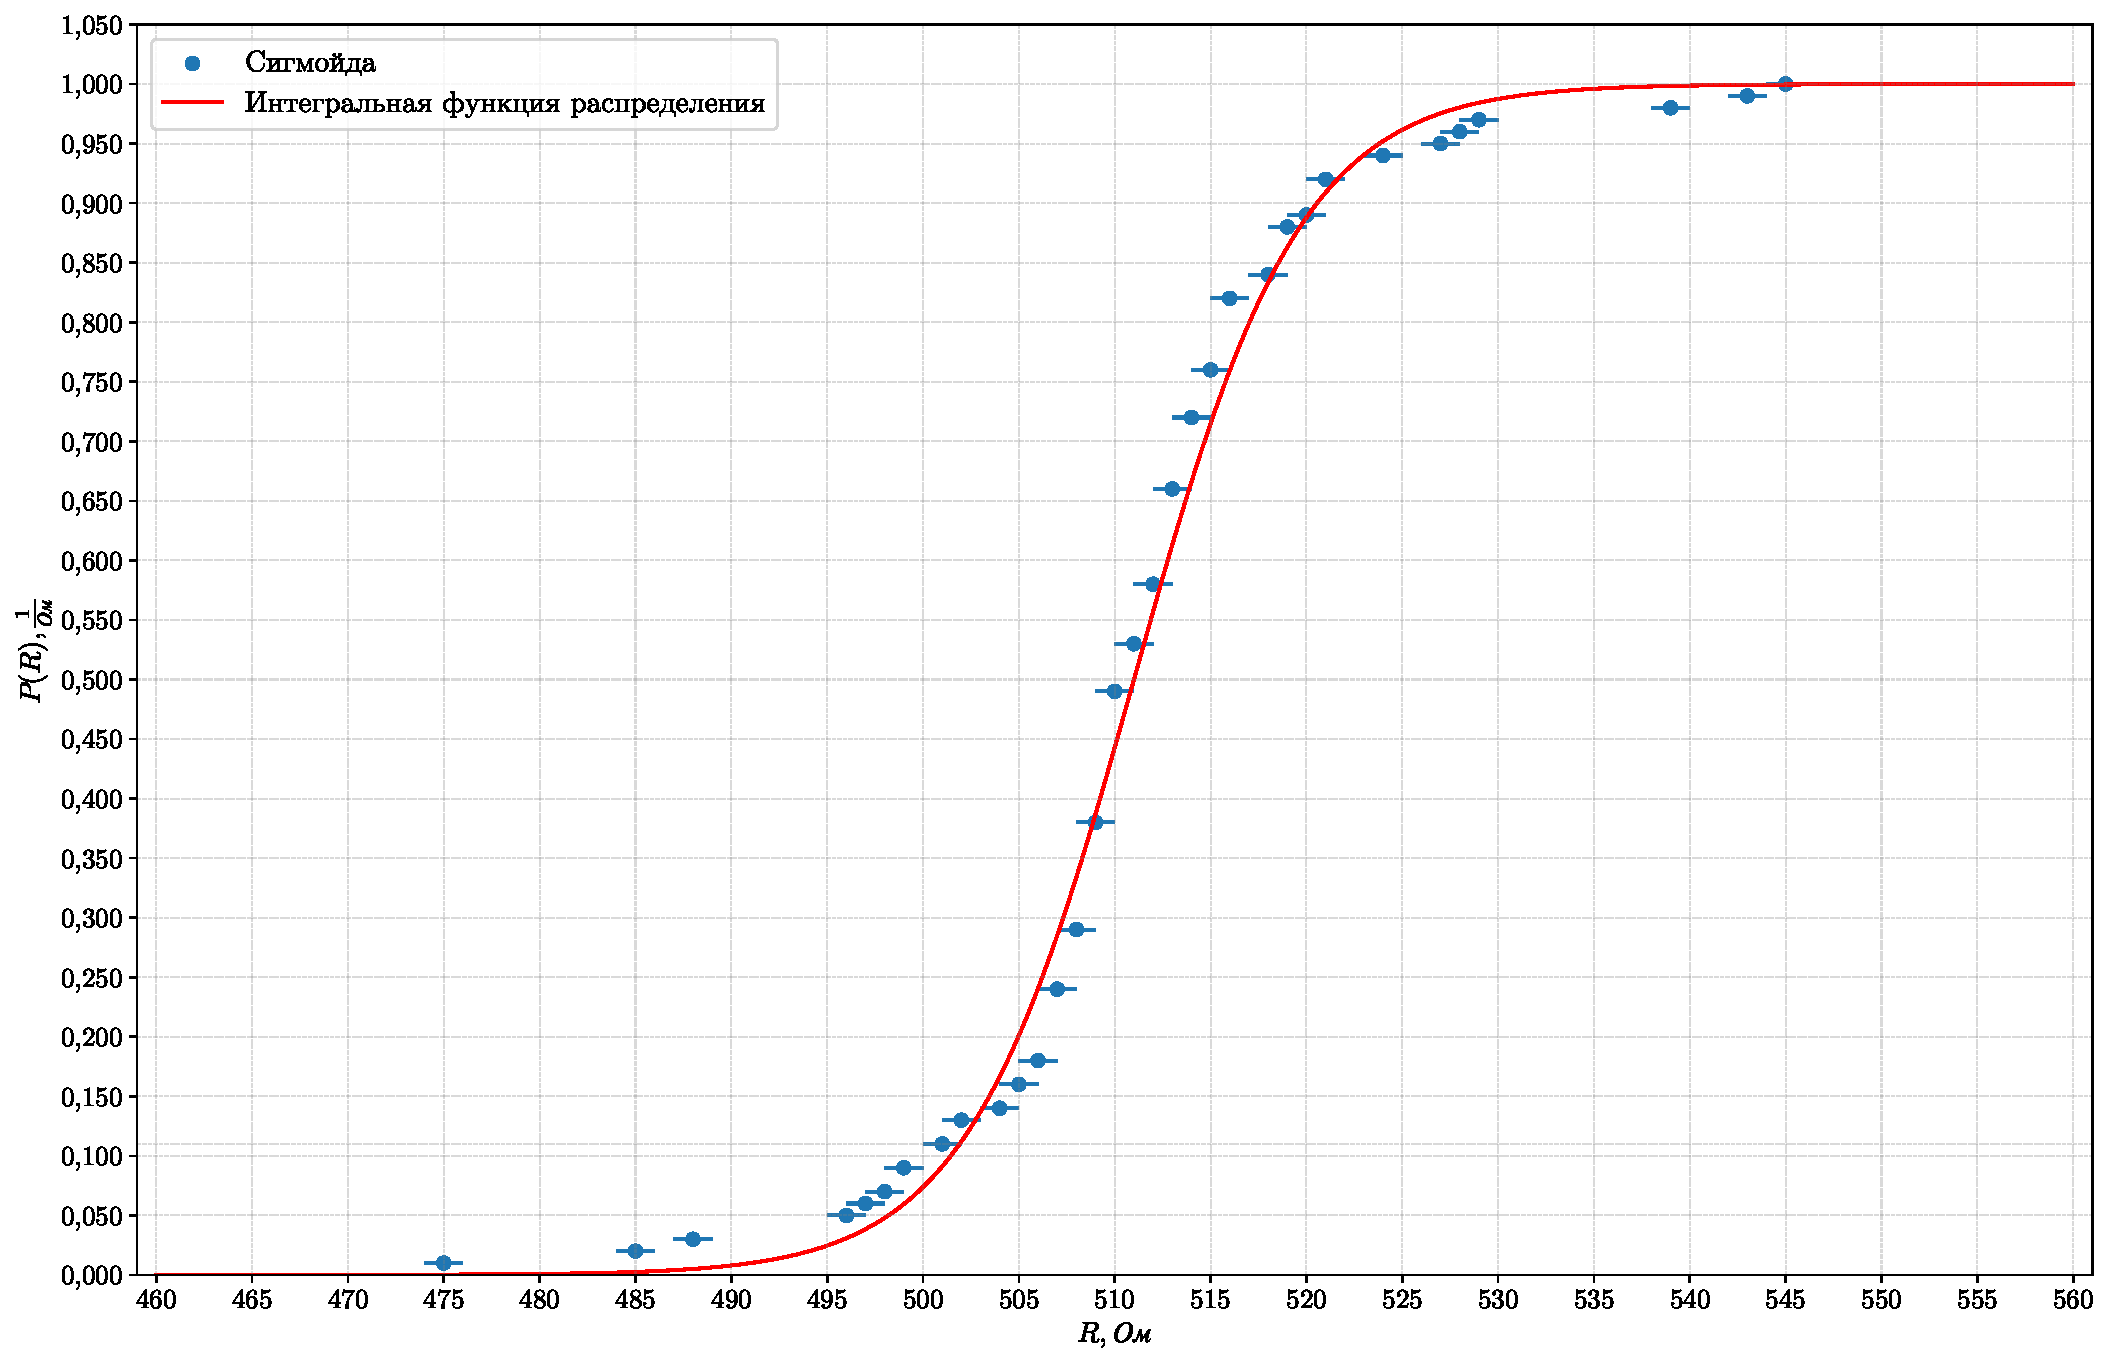
\includegraphics[angle = 270, width=0.8\textwidth]{ graph_3 } 
	\caption{График для опыта с резисторами $F(r)$}
	
	\label{fig:graph-3} 
\end{figure}

\begin{figure}[H] 
	\centering
	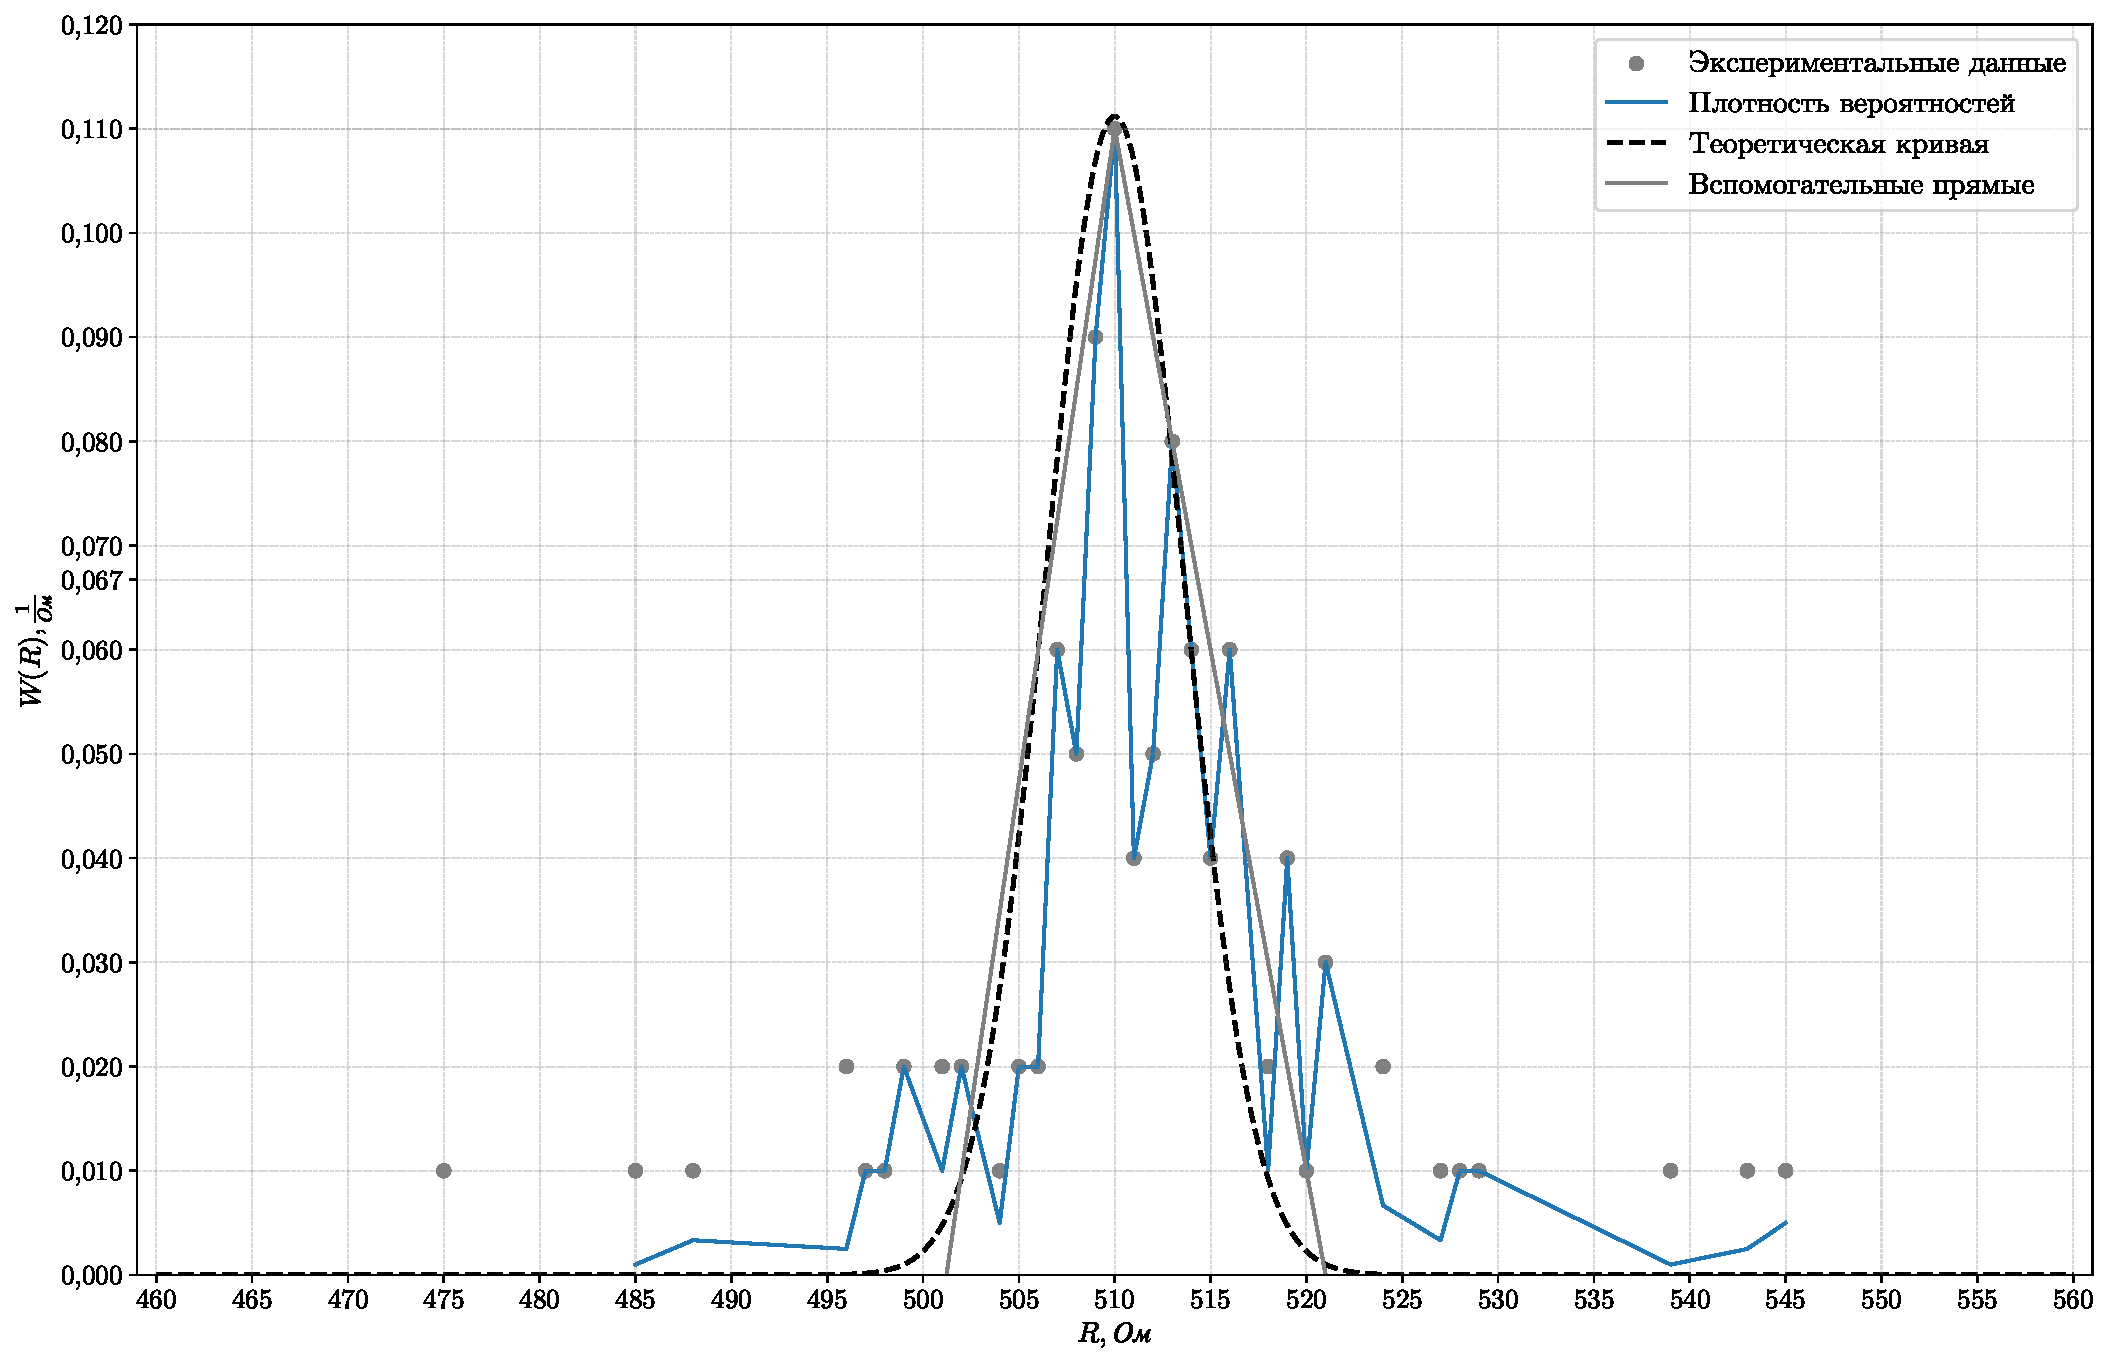
\includegraphics[angle = 270, width=0.8\textwidth]{ graph_4 } 
	\caption{График для опыта с резисторами (общий вид)}
	
	\label{fig:graph-4} 
\end{figure}
